\chapter{Week2 : Part A}

\begin{defnbox}[title=Validation vs.\ Verification]
\begin{itemize}
  \item \textbf{Validation} asks whether the requirements themselves are the right ones.
  \item \textbf{Verification} checks that the product actually satisfies those requirements.
\end{itemize}
\tcblower
The goal of testing is to find bugs so they can be fixed before release.
\end{defnbox}

\section{Testing: Different Levels}
\textit{(recap from CS-214)}

\begin{itemize}
  \item \textbf{Unit tests} exercise individual components or functions in isolation --- e.g.\ a user-input validation function.
  \item \textbf{Integration tests} exercise combinations of components together --- e.g.\ the login interface talking to the backend database.
  \item \textbf{System tests} exercise the complete, integrated software --- e.g.\ the entire app's functionality.
  \item \textbf{End-to-end tests} follow a full user journey from start to finish. Every e2e test is a system test, but not every system test is end-to-end.
  \item \textbf{Acceptance tests} exercise the product in real-world scenarios to confirm it meets stakeholders' requirements.
\end{itemize}

\subsection{Writing Good Unit Tests}

\begin{itemize}
  \item \textbf{Keep tests small, checking only one thing}
  \item \textbf{Keep tests independent of each other}
  \item \textbf{Decouple tests from the rest of the implementation}, as much as possible, especially around object creation
\end{itemize}

\section{The Cost of Bugs}

\textbf{More causes of increasing bug costs:}

\begin{itemize}
  \item \textbf{Technical debt}
  \begin{itemize}
    \item bug workarounds $\Rightarrow$ codebase becomes more complex and fragile
  \end{itemize}
  \item \textbf{Lost knowledge}
  \begin{itemize}
    \item the longer a bug lives, the more likely the original developers have moved on
  \end{itemize}
  \item \textbf{Entrenchment} --- the bug has become part of the interface
  \begin{itemize}
    \item other code and other systems come to depend on the buggy behavior, so eventually you can't fix it without breaking them
  \end{itemize}
\end{itemize}

\begin{center}
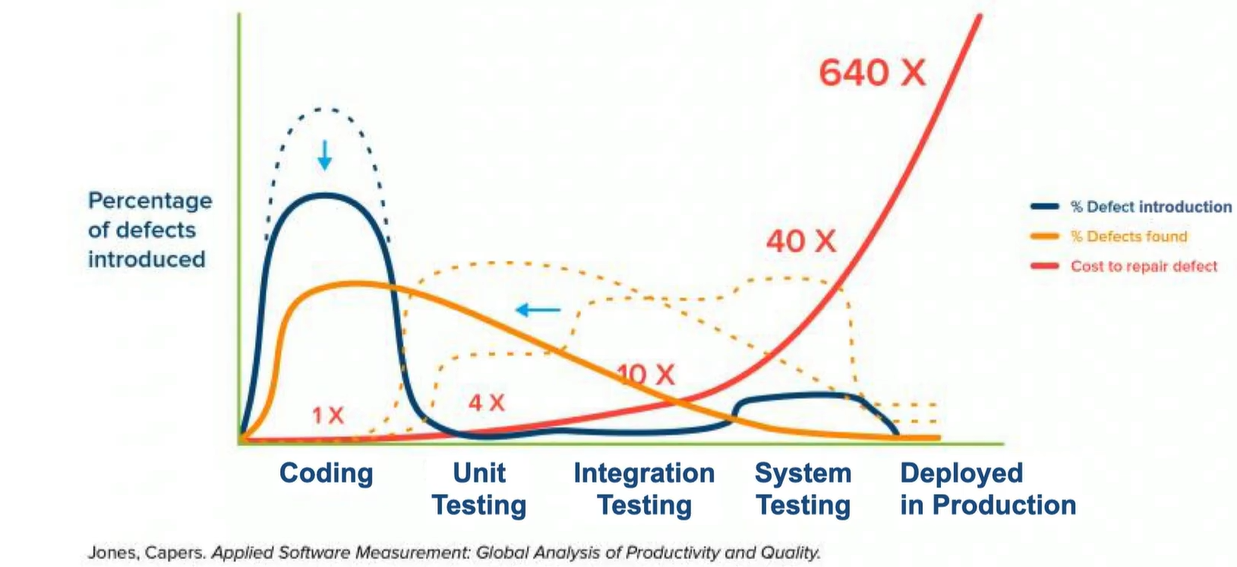
\includegraphics[width=\linewidth]{images/graphic-cost-bugs.png}
\end{center}

\section{How Well Can We Test?}

\begin{rembox}[title=Dijkstra's Law]
\itshape Program testing can be used to show the presence of bugs, but never to show their absence!
\par\hfill Edsger W. Dijkstra
\par\hfill \textit{Notes on Structured Programming} (1970)
\end{rembox}

\begin{itemize}
  \item Cannot test all behaviors (too many)
  \item \textbf{Goal of testing}
  \begin{itemize}
    \item identify bugs in order to fix them
    \item gain confidence in software quality
    \item statistically verify that program meets requirements
  \end{itemize}
  \item How do we tell how much testing we still need to do?
\end{itemize}

\section{Coverage Metrics}

\begin{itemize}
  \item \textbf{Statement coverage}
  \begin{itemize}
    \item easy to compute, easy to reason about
    \item a decent first-cut approximation of how good your tests are
  \end{itemize}
  \item \textbf{Branch coverage}
  \begin{itemize}
    \item more complicated but still doable
    \item a better estimate of the quality of your tests
    \item basis-set testing (cyclomatic complexity) gives us the sets for 100\% branch coverage
  \end{itemize}
  \item \textbf{Path coverage}
  \begin{itemize}
    \item impractical
    \item the perfect measure of how good your tests are
  \end{itemize}
\end{itemize}

\section{Technical Debt}

\begin{itemize}
  \item \textbf{Implied cost of additional rework caused by doing a hack}
  \begin{itemize}
    \item fixing hard-coded values, poorly structured code, coding-convention violations, \ldots
  \end{itemize}
  \item \textbf{Causes}
  \begin{itemize}
    \item Rushed timelines, incomplete requirements, lack of knowledge, legacy code, evolution
  \end{itemize}
  \item \textbf{Kinds of technical debt}
  \begin{itemize}
    \item Deliberate, Inadvertent, Bit Rot
  \end{itemize}
  \item \textbf{Managing technical debt}
  \begin{itemize}
    \item Recognize, Measure, Devise a repayment plan, Prevent
  \end{itemize}
\end{itemize}

\section{Code Smells}

\begin{itemize}
  \item \textbf{Code patterns that suggest a potential issue or problem}
  \begin{itemize}
    \item not bugs, just indicators of increased risks for future bugs, maintainability challenges, etc.
  \end{itemize}
\end{itemize}

\begin{multicols}{2}
\begin{itemize}
  \item Large Class
  \item Long Method
  \item Primitive Obsession
  \item Feature Envy
  \item Duplicated Code
  \item God Object
  \item Data Clumps
  \item Shotgun Surgery
  \item Lazy Class/Freeloader
  \item Speculative Generality
  \item Temporary Field
  \item Message Chains
  \item Middle Man
\end{itemize}
\end{multicols}

\begin{center}
\begin{minipage}[t]{0.48\linewidth}
\centering
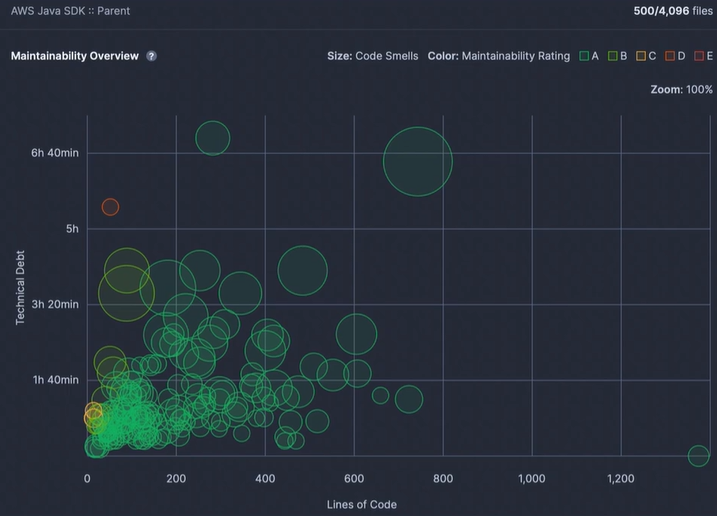
\includegraphics[width=\linewidth]{images/code-smell-A.png}
\end{minipage}\hfill
\begin{minipage}[t]{0.48\linewidth}
\centering
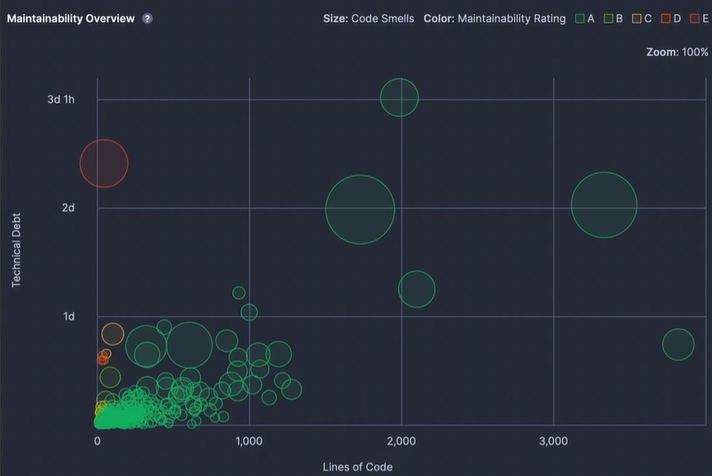
\includegraphics[width=\linewidth]{images/code-smell-B.png}
\end{minipage}
\end{center}

\begin{exbox}[title=Maintainability overview]
\small
Each bubble is one file: \textbf{lines of code} on the x-axis, \textbf{technical debt} (estimated time to fix) on the y-axis, \textbf{bubble size} is the number of code smells, and \textbf{color} is the maintainability rating (A, healthy, through E, critical).
\begin{itemize}[leftmargin=1.5em, itemsep=3pt]
  \item Most files cluster near the origin: small, low-debt, rated A --- the bulk of a healthy codebase.
  \item The outliers --- large bubbles, or bubbles shifted toward orange/red --- are the files worth refactoring first: many smells and/or high estimated debt relative to their size.
  \item The right-hand chart is the same view at a larger scale (debt in days rather than hours), showing how smells and debt compound as files grow.
\end{itemize}
\end{exbox}

\section{What Coverage Doesn't Catch}

\subsection{The Imperfection of Coverage}

\begin{itemize}
  \item High coverage $\Rightarrow$ well-exercised codebase $\nRightarrow$ freedom from defects
  \item \textbf{Coverage is an imperfect proxy metric for test quality}
  \begin{itemize}
    \item measures how much code is executed by tests, not how well they test the code
    \item does not measure the quality and importance of the test scenarios
  \end{itemize}
  \item \textbf{Challenge: Not all code is equal}
  \item \textbf{Challenge: Flaky tests}
  \item \textbf{Challenge: Contextual sensitivity}
  \begin{itemize}
    \item the more circumstances need to combine in order for a bug to manifest, the harder it is to anticipate and reveal them in testing (e.g., concurrency issues)
  \end{itemize}
\end{itemize}

\subsection{Smartphone Platform: Heterogeneity Challenges to Testing}

\begin{itemize}
  \item \textbf{Devices}
  \begin{itemize}
    \item device-specific or configuration-specific bugs
  \end{itemize}
  \item \textbf{Integration with external systems}
  \begin{itemize}
    \item you depend on the network!
    \item unexpected behavior can cause mobile app to misbehave
  \end{itemize}
  \item \textbf{Users}
  \begin{itemize}
    \item watch your input validation
  \end{itemize}
  \item \textbf{Sensors are finicky}
  \item \textbf{Interaction with system features}
\end{itemize}

\subsection{Testing Challenges: Non-Functional Requirements}

\begin{itemize}
  \item performance, security, usability, compatibility, etc.
  \item test coverage numbers do not capture these directly
  \begin{itemize}
    \item yet they can significantly impact user experience
  \end{itemize}
  \item static analysis tools
  \item performance and load testing
  \item security testing (both automated and manual)
  \item exploratory testing
\end{itemize}

\subsection{Careful What You Ask For}

\begin{warnbox}[title=An agent optimizes exactly the metric you name]
\begin{itemize}
  \item ask for ``increase coverage to 80\%'' and you get the two tests we opened with
  \item ask for tests of specific behaviors, and you get tests
\end{itemize}
\end{warnbox}

\begin{itemize}
  \item \textbf{For every test: what would have to break for this to fail (i.e., ``go red'')?}
  \begin{itemize}
    \item if you can't answer in one sentence, it isn't a test --- delete it
  \end{itemize}
  \item \textbf{Verify the suite, not the number}
  \begin{itemize}
    \item break your own code on purpose; if nothing goes red, your tests are decorative
  \end{itemize}
  \item \textbf{A coverage jump is a reason to look harder, not to celebrate}
  \begin{itemize}
    \item 40\% to 90\% in one afternoon could mean 40 plausible green tests nobody has read
  \end{itemize}
\end{itemize}

\section{Takeaways}

\begin{keybox}
\begin{itemize}
  \item \textbf{Coverage metrics}
  \begin{itemize}
    \item just an indicator, they do not ``sign off'' on software quality
    \item provide guidance: areas that need attention
  \end{itemize}
  \item \textbf{Tests are code}
  \begin{itemize}
    \item update tests as code evolves (e.g., every time you fix a bug, write a test for it)
    \item keep tests under version control
    \item run often
    \item should be of production quality
  \end{itemize}
  \item \textbf{Look at the big picture}
  \begin{itemize}
    \item consider technical debt, code smells, etc.
  \end{itemize}
\end{itemize}
\end{keybox}

